\chapter{Алгоритм последовательной генерации состояний}
\label{sec:seq-statespace}

\section{Алгоритм поиска в глубину}
\label{sec:seq-algo}

Для построения пространства состояний ПО Spin использует последовательный поиск в
глубину, который можно представить следующим псевдокодом:

\begin{lstlisting}[style=pseudocode]
Visited = []

def StateSpaceDFS(state):
    if not state in Visited:
        Visited <- state
        for each new_state in Next(state):
            StateSpaceDFS(new_state)

StateSpaceDFS(initial_state)
\end{lstlisting}

Для получения $Next(s)$ вычисляются условия выполнимости текущих инструкций всех
процессов, присутствующих в $s$ (отсюда мы получаем множество незаблокированных процессов
$P_{ready}(s)$), после чего для каждого процесса $P$ из $P_{ready}(s)$ генерируется новое
состояние, получающееся в результате выполнения его текущей инструкции (номер которой
хранится в $IP_P$). Это можно представить в виде псевдокода как:

\begin{lstlisting}[style=pseudocode]
def Next(state):
    Next = []
    for each process in state:
        if Executable(process):
            new_state = Copy(state)
            Step(new_state, process)
            Next <- new_state
\end{lstlisting}

Здесь \Code{Executable}~--- функция проверки выполнимости текущей инструкции процесса, а
\Code{Step}~--- функция трансформации состояния при выполнении текущей инструкции
выбранного процесса.

\section{Хранение посещенных состояний}
\label{sec:state-hashing}

При генерации каждого состояния делается проверка, было ли оно уже посещено ранее
(т.е. находится в множестве \Code{Visited}) и добавление в этом множество в противном
случае. Для эффективного поиска состояния \Code{Visited} представляется в виде
хэш-таблицы.

По мере роста степени загрузки хэш-таблицы с большой вероятностью возникают коллизии; в
соответствии с парадоксом <<дней рождения>>, если в таблице на миллион элементов хранится
2500 ключей (т.е. степень заполненности составляет лишь 0.0025\%), вероятность совпадения
хэш-кодов хотя бы двух из них составляет 95\%, поэтому необходим алгоритм разрешения
коллизий.

%\paragraph{Закрытая адресация}
%\label{sec:closed-addressing}

При <<закрытой адресации>> (хэш-таблице со списками), показанной на
рис.~\ref{fig:hash-addressing} слева, каждый элемент хэш-таблицы представляет собой список
всех состояний, хэш-коды которых совпадают и приходятся на этот элемент. При поиске
состояния $s$ все состояния в списке сравниваются (побайтово) с $s$, пока не будет
обнаружено совпадение.

При размере таблицы $N$ и количестве записей в ней $M$, вероятность коллизии при каждом
обращении составляет $\frac{M}{N}$ (т.е. растет линейно с $M$). Поскольку длина списка
состояний в каждой ячейке в среднем не превосходит 2 даже при заполненности таблицы
(отношении количества хранимых состояний к количесту ячеек в таблице), близкой к 1, время
поиска в хэш-таблице с закрытой адресацией растет линейно с ростом ее
заполненности.~\cite{CDataStructures}.

%\paragraph{Открытая адресация с линейными пробами}
%\label{sec:open-linear-probing}

В этом случае каждый элемент хранит ровно одно состояние
(см. рис.~\ref{fig:hash-addressing} справа). При поиске или сохранении состояния, если
элемент $i = hash(s)$ занят другим состоянием (не совпадающим с $s$), проверяются элементы
с номерами $i + a, i + 2 \cdot a, i + 3 \cdot a, \ldots$ до тех пор, пока не будет найдено
нужное состояние либо не будет обнаружена свободная ячейка (это означает, что $s$
отсутствует в хэш-таблице). Число $a$ должно быть взаимно просто с размером
хэш-таблица~--- это позволяет гарантировать, что при полностью заполненной хэш-таблице
каждый элемент будет проверен хотя бы один раз.

Недостаток этого алгоритма в том, что элементы имеют тенденцию <<скапливаться>> в
определенных областях, поскольку коллизия в одной ячейке сразу повышает вероятность
коллизии в соседней, коллизия в ней приводит к коллизии в следующей\etc

\begin{figure}[ht]
  \centering
  \begin{tabular}{cc}
    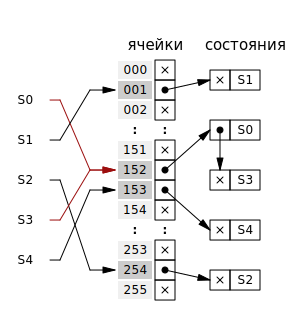
\includegraphics{../graphics/hash-closed}
    &
    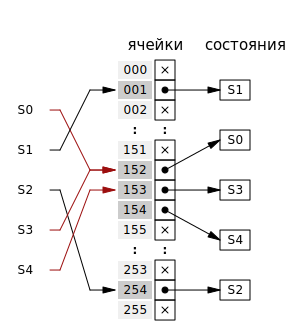
\includegraphics{../graphics/hash-open}
  \end{tabular}
  \caption{Различные схемы адресации в хэш-таблице}
  \label{fig:hash-addressing}
\end{figure}

%\paragraph{Открытая адресация с квадратичными пробами}
%\label{sec:open-quadratic-probing}

Для решение проблемы предыдущего метода предлагается иная последовательность проб: при
коллизии элемента в ячейке $i$ проверяются ячейки с номерами $i + a + b, i + 4 \cdot a + 2
\cdot b, i + 9 \cdot a + 3\cdot b, \ldots$. Эти номера составляют квадратичную прогрессию,
отсюда и название. Преимуществом квадратичных проб над линейными является меньшая
кластеризация коллизий при сохранении свойства локальности: просматриваемые при
поиске/вставке первые 3-4 состояний находятся достаточно близко друг к другу, чтобы
попадать в одну строку кэша.

%\paragraph{Двойное хэширование}
%\label{sec:open-double-hashing}

Другим подходом к устранению кластеризации коллизий является использование вторичной
функции хэширования, $hash'$. В случае коллизии просматриваются состояния $i + hash'(a), i
+ 2\cdot hash'(a), \ldots$. Однако, данный подход полностью лишен свойства локальности (в
случае коллизии следующее же проверяемое состояние уже выходит за пределы строки кэша с
только что выбранным), поэтому используется реже.

Общей проблемой всех методов открытой адресации заключается в том, что хранить в ней
больше состояний, чем позволяет размер таблицы, невозможно (в то время как при закрытой
адресации размер таблицы не является ограничением). Более того, когда степень
заполненности таблицы превышает 80\%, производительность поиска начинает резко падать,
уменьшаясь на порядок при заполненности в 90\%. Это связано с тем, что средняя длина
цепочки просматриваемых при коллизии состояний растет линейно вместе с заполненностью
таблицы $\frac{M}{N}$, а не остается константой, как при закрытой адресации.

Преимущество открытой адресации в том, что нет необходимости хранить списки состояний,
следовательно, расход памяти меньше. Особенно это важно для моделей, состояние занимает
небольшой объем памяти (порядка 20--30 байт), потому что в этом случае на 64-битной
архитектуре экономия будет составлять 25--40\%. В то же время для моделей с состоянием
большого объема открытая адресация дает незначительное преимущество, и при высокой
заполненности хэш-таблицы использование закрытой адресации предпочитетельно.

\section{Проблема роста числа состояний}
\label{sec:state-explosion}

Последовательное построение пространства состояний $S$ с ростом размера модели быстро
становится невозможным из-за нехватки памяти для хранения множества достигнутых состояний
(\Code{Visited}). В табл.~\ref{tab:models-statecount} приведены данные для двух моделей:
модели задачи об обедающих философов из раздела~\ref{sec:promela} и более приближенной к
реальным задачам модели RIP-протокола на 4 сетевых маршрутизаторах.

\begin{table}
  \centering
  \begin{tabular}{|r|l|l|}
    \hline
    Модель                  & Состояний         & Переходов       \\
    \hline
    Философы (5)            & $2.8 \cdot 10^4$  & $4.2 \cdot 10^4$ \\
    Философы (7)            & $3.6 \cdot 10^5$  & $6.0 \cdot 10^5$ \\
    RIP (4 маршрутизатора)  & $1.6 \cdot 10^8$  & $4.8 \cdot 10^9$ \\
    \hline
  \end{tabular}
  \caption{Количество состояний и переходов в различных моделях}
\label{tab:models-statecount}
\end{table}

Из табл. \ref{tab:models-statecount} видно, что для реальных моделей традиционный подход
становится проблематичен: к примеру, модель RIP-протокола с 5-ю маршрутизаторами потребует
уже более 100 Гб оперативной памяти для хранения пространства состояний.

Существует ряд подходов, решающих данную проблему. Среди них можно выделить:

\begin{itemize}
\item методы оптимизации, уменьшающие количество генерируемых и хранимых состояний;
\item методы оптимизации, уменьшающие расход памяти на хранение пространства состояний;
\end{itemize}

Далее в разделах~\ref{sec:partial-order-reduction}--\ref{sec:state-compression} описан ряд
таких методов, используемых ПО Spin.

\section{Метод сокращения частных порядков}
\label{sec:partial-order-reduction}

Сокращение частных порядков (\Term{partial order reduction})~\cite{POD} относится к первой
группе: оно уменьшает количество генерируемых состояний. Данный метод использует тот факт,
что зачастую порядок выполнения двух переходов в различных процессах не оказывает влияния
на результат проверки.

Пример показан на рис.~\ref{fig:partial-order-reduction} слева: допустим, нас интересует
выполнение свойства $p$ в каждом из состояний системы. $\alpha$ и $\beta$~--- два перехода
различных процессов $P_{\alpha}$ и $P_{\beta}$, которые оба возможны в состоянии $s_0$
(т.е. $P_{\alpha}$ и $P_{\beta}$ не заблокированы). При этом переход $\beta$ нарушит
свойство $p$. В том случае, если выполнение свойства $p$ не зависит от перехода $\alpha$,
порядок выполнения этих двух переходов не важен, следовательно, генерацию состояния $s_2$
можно предотвратить (на рис.~\ref{fig:partial-order-reduction} справа).

\begin{figure}[ht]
  \begin{tabular}{p{0.4\textwidth}p{0.2\textwidth}p{0.2\textwidth}}
  \begin{tikzpicture}[->,>=stealth',auto,node distance=4cm,semithick]
    \tikzstyle{every state}=[fill=none,draw=black,text=black]
    \node[state]     (A)                    {$s_0:~~p~$};
    \node[state]     (B) [below right of=A] {$s_1:~~p~$};
    \node[state]     (C) [below left  of=A] {$s_2:~\neg p$};
    \node[state]     (D) [below right of=C] {$s_3:~\neg p$};
    
    \path (A) edge node {$\alpha$} (B)
              edge node {$\beta$}  (C)
          (B) edge node {$\beta$}  (D)
          (C) edge node {$\alpha$} (D);
  \end{tikzpicture}
  & 
  &
  \begin{tikzpicture}[->,>=stealth',auto,node distance=4cm,semithick]
    \tikzstyle{every state}=[fill=none,draw=black,text=black]
    \node[state]          (A)                    {$s_0:~p~$};
    \node[state]          (B) [below right of=A] {$s_1:~p~$};
    \node[state]          (D) [below left  of=B] {$s_3:~\neg p$};
    
    \path (A) edge node {$\alpha$} (B)
          (B) edge node {$\beta$}  (D);
  \end{tikzpicture}
  \end{tabular}
  \caption{Демонстрация сокращения частных порядков}
  \label{fig:partial-order-reduction}
\end{figure}

Сокращение частных порядков возможно далеко не для любых пар переходов, допустимых в
данном состоянии:

\begin{itemize}
\item переходы не должны влиять на выпонимость друг друга
\item (коммутативность) оба перехода должны приводить к одному и тому же состоянию
  вне зависимости от порядка выполнения: $Next(Next(s_0)) = \{ s_3 \}$
\end{itemize}

В случае, если два процесса обращаются к глобальным переменным и/или
используют каналы для взаимодействия, множество переходов, для которых
допустимо сокращение частных порядков, существенно уменьшается. Кроме
того, проверка на наличие циклов делает СЧП невозможным. Однако, в тех
случаях, когда это допустимо, ПО Spin применяет метод СЧП для
уменьшения пространства состояний.

% http://tele.informatik.uni-freiburg.de/Teaching/ss02/dres/dres.part8.pdf

\section{Использование битового хэширования состояний}
\label{sec:bit-hashing}

При битовом хэширование состояний (\Term{bit-state hashing})~\cite{BitHash1} вместо
традиционной хэш-таблицы для хранения состояний используется битовая таблица. Каждое
состояние $s$ представлено в ней битом с номером $i = hash(s)$. Нулевой бит
означает, что состояние еще не было достигнуто, единичный — было. При этом вся
используемая память отводится под хэш-таблицу (сами состояния не хранятся). При размере
состояния в 20-30 байт это позволяет хранить в 160-240 больше состояний, чем при
традиционном подходе.

К сожалению, коллизии в этом случае обнаружить невозможно -- состояния будут просто
<<теряться>>, поэтому приходится просто полагаться на то, что коллизий не возникнет (для
этого надо обеспечить низкую степень заполненности таблицы) или что <<потерянные>>
состояния не повлияют на итог. Такой подход сильно снижает надежность получаемого
результата, поэтому в чистом виде битовое хэширование используется крайне редко.

Пусть под хэш отводится $m$ бит ($M = 2^m$~--- количество бит в хэш-таблице), $N$~---
число состояний в $S$. При $N < M$, первое добавляемое в хэш состояние имеет нулевую
вероятность коллизии, последнее -- $\frac{N - 1}{M}$, отсюда усредненная по всем
состояниям вероятность коллизии
\begin{equation}
  \label{eq:bithash-single-coll1}
  P_1 \leq \frac{1}{N\cdot M} \sum_{i=0}^{N-1}i = \frac{N - 1}{2\cdot M} \leq 2^{n - m - 1}.
\end{equation}
Ожидаемое покрытие пространства состояний составляет $(1 - P_1)\cdot 100\%$.

При $N \geq M$, т.е. когда число состояний больше числа доступных бит в таблице,
возникновение как минимум $(N - M)$ коллизий неизбежно, поэтому
\begin{equation}
  \label{eq:bithash-single-coll2}
  P_1 \geq 1 - 2^{(m-n)}.
\end{equation}

\paragraph{Использование нескольких бит}
\label{sec:multi-bit-hashing}

Для улучшения покрытия пространства состояний в \cite{BitHash1} предлагается использовать
несколько независимых хэш-функций. Каждое состояние имеет, таким образом, $h$ индексов
($i_1 = hash_1(s), i_2 = hash_2(s) \ldots i_h = hash_h(s)$) и считается найденным в
хэш-таблице только в том случае, если все биты $i_1, i_2 \ldots i_h$ установлены. В ПО
Spin используется именно этот подход, при этом $h$ рекомендуется выбирать равным 2 либо
3.~\cite{SpinRoot}

В случае $h \cdot N < M$, усредненная вероятность коллизий, согласно~\cite{BitHash1},
\begin{equation}
  \label{eq:bithash-multi-coll1}
  P_h \leq \frac{1}{N} \sum_{i=0}^{N-1} (\frac{h \cdot i}{M})^h \leq \frac{(2 h)^h}{h+1} (P_1)^h,
\end{equation}
что при $h = 2$ дает 
\begin{equation}
  \label{eq:bithash-2bit-coll1}
  P_h \leq \frac{16}{3} 2^{2(n -m - 1)}.
\end{equation}

При $h \cdot N \geq M$, усредненная вероятность коллизий 
\begin{equation}
  \label{eq:bithash-multi-coll2}
  P_h \leq 1 - \frac{M}{h \cdot N} = 1 - \frac{1}{h} 2^{m - n}
\end{equation}
и по-прежнему не меньше, чем в (\ref{eq:bithash-single-coll2}).

Из исследований в~\cite{BitHash1} следует, что $h$ следует подбирать таким, чтобы
выполнялось $h \cdot N \leq M$, в противном случае ожидаемое покрытие падает в сравнении с
меньшим значением $h$. Например, при $M/3 < N < M/2$ предпочтительно использовать 2
хэш-функции, при $M/4 < N < M/3$~--- 3, а в случае $N > M/2$ любые $h > 1$ дают худшее
покрытие, чем $h = 1$.

\paragraph{Вторичное хэширование (hashcompact)}
\label{sec:hashcompact}

Еще один альтернативный подход под названием \Term{hashcompact} (в русской литературе
перевод не встречается, можно перевести как <<вторичное хэширование>>) предлагается
в~\cite{Wolper}. В нем предлагается хранить в хэш-таблице вместо самих состояний их
хэш-коды большей, чем у индексов хэш-таблицы, разрядности (например, 64 бита), полученные
при помощи независимой от основной хэш-функции $hash^*(s)$.

Максимальное число хранимых в этом случае состояний равняется
$M/64$. Согласно~\cite{BitHash1}, hashcompact дает лучшее, чем битовое хэширование с $h =
2$, покрытие при
\begin{equation}
  \label{eq:hashcompcat-coverage-optima}
  \frac{M}{100} \leq N \leq \frac{M}{64}.
\end{equation}
При значениях $N$, меньших $M/100$, битовое хэширование с двумя функциями обеспечивает
лучшее покрытие, а при $N > M/64$ покрытие hashcompcat резко падает.~\cite{Wolper}

%!!! Может, вставить тут график с их сравнением?..

\section{Метод сжатия хранимых состояний}
\label{sec:state-compression}

% http://citeseerx.ist.psu.edu/viewdoc/summary?doi=10.1.1.38.308
% http://citeseerx.ist.psu.edu/viewdoc/download?doi=10.1.1.38.308&rep=rep1&type=pdf

Альтернативным способом, позволяющим уменьшить требуемый объем памяти ценой уменьшения
скорости генерации, является сжатие хранимых состояний.

Можно предложить следующие способы сжатия состояний:

\begin{enumerate}
\item Сжатие при помощи кодов Хаффмана. Согласно исследованию из \cite{StateCompr}, в ходе
  которого было рассмотрен ряд моделей из реальных задач, в состояниях преобладают байты с
  малыми значениями, т.е. распределение значений байт в состояниях неравномерно; это
  делает коды Хаффмана хорошо применимыми. Недостатком кодов Хаффмана является
  существенное замедление работы (до 200\%).

\item <<Рекурсивная индексация>> состояний использует тот факт, что состояние $s$ включает
  в себя набор состояний отдельных процессов $s_{P_0}, s_{P_1}, ... s_{P_N}$; поскольку
  размер пространства состояний отдельно взятого процесса гораздо меньше, чем для всей
  системы, можно хранить локальные состояния процессов в отдельной хэш-таблице. При этом в
  глобальном состоянии по-прежнему хранятся значения глобальных переменных и содержимое
  каналов; все локальные состояния выносятся во вторичную хэш-таблицу, а их индексы
  хранятся в глобальном состоянии вместо них самих. Согласно \cite{StateCompr}, выгоднее
  использовать одну вторичную хэш-таблицу вместо отдельных таблиц для каждого типа
  процессов (proctype). Недостатком данного подхода является необходимость заранее (на
  этапе генерации кода или при его инициализации) выбирать, сколько бит в состоянии
  отводить под индексы в хэш-таблицу локальных состояний (если впоследствии окажется, что
  размер вторичной таблицы недостаточен для хранения всех состояний, ее увеличение будет
  невозможно, так как потребовало бы пересчета всех уже сгенерированных состояний).
\end{enumerate}

В \cite{StateCompr} предлагается еще ряд методов сжатия, выгодных для частных случаев
задач, однако в рамках данной работы они не рассматриваются.

%%% Local Variables: 
%%% mode: latex
%%% TeX-master: "thesis"
%%% End: 
